\documentclass{article}
\usepackage[utf8]{inputenc}
\usepackage{graphicx}
\usepackage{geometry}
\geometry{margin=.5in}

\title{ECON 1123 Final Exam Cheatsheet}

\begin{document}

\maketitle

\section{Statistics}

\begin{itemize}
    \item Variance of a sum:
    $$Var(aX + bY) = a^2var(X) + b^2var(Y) + 2ab \cdot cov(X, Y)$$
    \item Significance: A measure is significant at the 5\% level if:
    \begin{itemize}
        \item The test statistic is larger than the 5\% critical value for the test. OR 
        \item The p-value is less than .05 OR
        \item The 95\% confidence interval does not include 0.
    \end{itemize}
    \item 95 \% Confidence Interval:
    \begin{itemize}
        \item An interval that will contain the true value of a point estimate in 95\% of repeated samples.
        \item A set of values that cannot be rejected at a 5\% level with the data we have.
    \end{itemize}
\end{itemize}

\section{Interpretations}
 

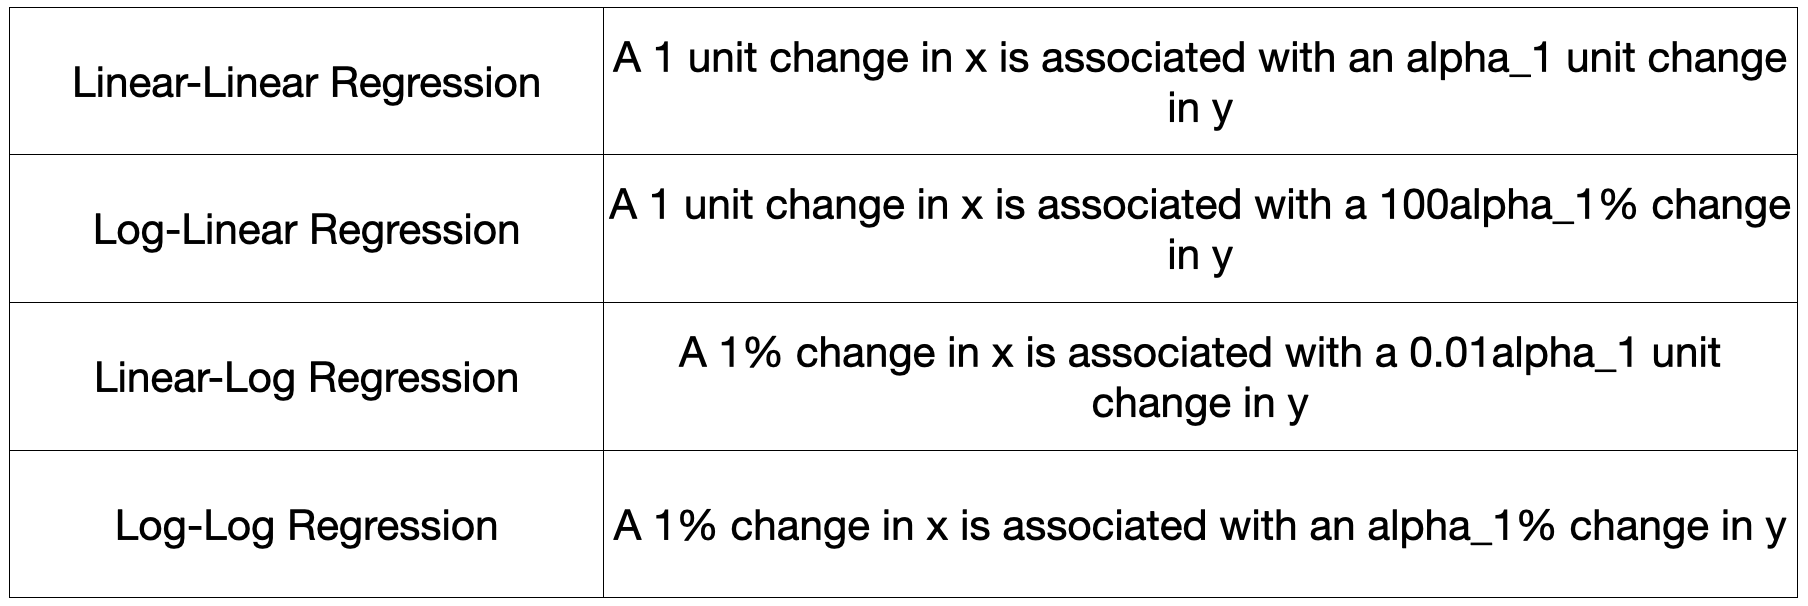
\includegraphics[scale=.4]{log_table.png}

\section{Omitted Variable Bias}

$$Y = \alpha_0 + \alpha_1 X \mbox{ (Short Form)}$$
$$Y = \beta_0 + \beta_1 X + \beta_2 W \mbox{ (Long Form)}$$
$$W = \gamma_0 + \gamma_1 X$$

\begin{itemize}
    \item Omitted variable must be something correlated with $X$ and $Y$, but should not be part of a causal channel.
    \item Steps:
    \begin{enumerate}
        \item Choose a valid omitted variable
        \item Sign $\beta_2$ (correlation between omitted variable and $Y$)
        \item Sign $\gamma_1$ (correlation between omitted variable and $X$)
        \item Use the above two to sign the bias ($bias = \beta_2 \times \gamma_1$)
        \item Use the above to decide if we have overstated or understated the causal effect.
    \end{enumerate}
    \item HINT: if $\alpha_1$ and $bias$ have the same signs, you have overstaded the causal effect. If they have different signs, you have understaded causal effect.
\end{itemize}

\section{Threats to Validity}
\begin{itemize}
    \item Internal: Have we correctly estimated coefficients and standard errors within our sample?
    \begin{itemize}
        \item Omitted Variable Bias
        \item Functional Form Bias
        \item Measurement Error (in $X$) (Attenuation Bias)
        \item Bad Controls
        \item Sample Selection Bias
        \item Simultaneous Causality Bias
        \item Wrong Standard Errors

        All of the above except the last one are a result of conditional mean independence being violated, meaning after controls, the variable of interest is as good as randomly assigned.
    \end{itemize}
    \item External: Can our results be extended to other populations?
    \begin{itemize}
        \item Different place, time, group of people, etc.
    \end{itemize}
\end{itemize}

\section{Standard Errors}

\begin{itemize}
    \item Heteroskedasticity-Robust vs. Pooled: Pooled standard errors only work when variance is constant across our dataset. HR standard errors work either way.
    \item Clustered SEs: We use clustered standard errors to account for serial correlation in the data. This is necessary when data points are not independent of each other, as in panel data. We always cluster at the level of policy change (change in treatment).
    \item Newey-West SEs: Newey-West standard errors account for autocorrelation in the error terms. You don't need to use these if you're already accounting for autocorrelation in your regression!
\end{itemize}

\section{Instrumental Variables}
\begin{itemize}
    \item Instrument $Z$, Treatment $X$, outcome $Y$
    \item First-stage: $X = \pi + \pi_1 Z$
    \item Reduced-Form: $Y = \alpha_0 + \alpha_1 Z$
    \item $\beta_1 = \frac{\alpha_1}{\pi_1}$
    \item Requirements for Valid Instrument:
    \begin{itemize}
        \item Relevance: $Z$ plausibly has impact on $X$. We measure this with first-stage f-statistic. If there is just one instrument, we can calculate this using the first-stage regression: $$F = \left(\frac{\pi_1}{SE(\pi_1)}\right)^2$$ and the critical value is 23.1
        \item Exogeneity:
        \begin{itemize}
            \item As good as randomly assigned: With any necessary controls, the instrument is as good as randomly assigned.
            \item Instrument only effects outcome through treatment. Instrument cannot affect outcome directly and cannot affect it through another variable.
        \end{itemize}
    \end{itemize}
    \item LATE vs. ATE: 
    \begin{itemize}
        \item Local average treatment effect is measured by 2SLS and is a weighted average where compliers have greater weights than non-compliers.
        \item Compliers (grasshoppers) are those for whom the instrument affects the treatment. Non-compliers (ants) are those for whome the instrument does not affect the treatment.
        \item Steps to LATE vs. ATE Problem:
        \begin{enumerate}
            \item Eliminate 3 cases where LATE = ATE. 
            \begin{enumerate}
                \item $\pi_i$ is constant, meaning compliance levels are the same for everyone.
                \item $\beta_1$ is constant, meaning the treatment effect is the same for everyone.
                \item $cov(\pi_1, \beta_1) = 0$, meaning being a complier or non-complier is not related to the treatment effect in any way.
            \end{enumerate}
            \item Identify who the compliers and non-compliers are. (These can be a smaller group within compliers or non compliers, eg. you could say rich people are more or less likely to be compliers)
            \item State whether the treatment effect (effect of $X$ on $Y$) is larger (in absolute value) for compliers or non-compliers. Make sure you are ignoring the instrument here, and only looking at the effect of $X$ on $Y$.
            \item Finally, use the above to state whether LATE is bigger than or smaller than ATE.
        \end{enumerate}
    \end{itemize}
\end{itemize}

\section{Cumulative Impluse Response Functions}
\begin{itemize}
    \item For a regression of the form:
    $$Y_{it} = \beta_0 + \beta_1 X_{it} + \beta_2 X_{it - 1} + \beta_3 X_{it - 2} $$
    \item Where $\Delta X_{it} = X_{it} - X_{it-1}$
    \item Then for the additional regression:
    $$Y_{it} = \delta_0 + \delta_1 \Delta X_{it} + \delta_2 \Delta X_{it - 1} + \delta_3 X_{it - 2} $$
    \item $\delta_1 = \beta_1$, $\delta_2 = \beta_1 + \beta_2$, and $\delta_3 = \beta_1 + \beta_2 + \beta_3$
    \item Long-Run Cumulative Effect: $\beta_1 + \beta_2 + ...$, or $\delta_n$.
    \item Cumulative Impulse Response Function. Graphing number of lags on the x axis, and total cumulative effect to that point on the y.
\end{itemize}





\end{document}